%%%%%%%%%%%%%%%%%%%%%%%%%%%%%%%%%%%%%%%%%
% Lachaise Assignment
% LaTeX Template
% Version 1.0 (26/6/2018)
%
% This template originates from:
% http://www.LaTeXTemplates.com
%
% Authors:
% Marion Lachaise & François Févotte
% Vel (vel@LaTeXTemplates.com)
%
% License:
% CC BY-NC-SA 3.0 (http://creativecommons.org/licenses/by-nc-sa/3.0/)
% 
%%%%%%%%%%%%%%%%%%%%%%%%%%%%%%%%%%%%%%%%%

%----------------------------------------------------------------------------------------
%	PACKAGES AND OTHER DOCUMENT CONFIGURATIONS
%----------------------------------------------------------------------------------------

\documentclass{article}

%%%%%%%%%%%%%%%%%%%%%%%%%%%%%%%%%%%%%%%%%
% Lachaise Assignment
% Structure Specification File
% Version 1.0 (26/6/2018)
%
% This template originates from:
% http://www.LaTeXTemplates.com
%
% Authors:
% Marion Lachaise & François Févotte
% Vel (vel@LaTeXTemplates.com)
%
% License:
% CC BY-NC-SA 3.0 (http://creativecommons.org/licenses/by-nc-sa/3.0/)
% 
%%%%%%%%%%%%%%%%%%%%%%%%%%%%%%%%%%%%%%%%%

%----------------------------------------------------------------------------------------
%	PACKAGES AND OTHER DOCUMENT CONFIGURATIONS
%----------------------------------------------------------------------------------------

\usepackage{amsmath,amsfonts,stmaryrd,amssymb} % Math packages

\usepackage{enumerate} % Custom item numbers for enumerations

\usepackage{subcaption}
\usepackage{cleveref}
\usepackage[ruled]{algorithm2e} % Algorithms

\usepackage[framemethod=tikz]{mdframed} % Allows defining custom boxed/framed environments

\usepackage{listings} % File listings, with syntax highlighting
\lstset{
	basicstyle=\ttfamily, % Typeset listings in monospace font
}

%----------------------------------------------------------------------------------------
%	DOCUMENT MARGINS
%----------------------------------------------------------------------------------------

\usepackage{geometry} % Required for adjusting page dimensions and margins

\geometry{
	paper=a4paper, % Paper size, change to letterpaper for US letter size
	top=2.5cm, % Top margin
	bottom=3cm, % Bottom margin
	left=2.5cm, % Left margin
	right=2.5cm, % Right margin
	headheight=14pt, % Header height
	footskip=1.5cm, % Space from the bottom margin to the baseline of the footer
	headsep=1.2cm, % Space from the top margin to the baseline of the header
	%showframe, % Uncomment to show how the type block is set on the page
}

%----------------------------------------------------------------------------------------
%	FONTS
%----------------------------------------------------------------------------------------

\usepackage[utf8]{inputenc} % Required for inputting international characters
\usepackage[T1]{fontenc} % Output font encoding for international characters

%\usepackage{XCharter} % Use the XCharter fonts

%----------------------------------------------------------------------------------------
%	COMMAND LINE ENVIRONMENT
%----------------------------------------------------------------------------------------

% Usage:
% \begin{commandline}
%	\begin{verbatim}
%		$ ls
%		
%		Applications	Desktop	...
%	\end{verbatim}
% \end{commandline}

\mdfdefinestyle{commandline}{
	leftmargin=10pt,
	rightmargin=10pt,
	innerleftmargin=15pt,
	middlelinecolor=black!50!white,
	middlelinewidth=2pt,
	frametitlerule=false,
	backgroundcolor=black!5!white,
	frametitle={Command Line},
	frametitlefont={\normalfont\sffamily\color{white}\hspace{-1em}},
	frametitlebackgroundcolor=black!50!white,
	nobreak,
}

% Define a custom environment for command-line snapshots
\newenvironment{commandline}{
	\medskip
	\begin{mdframed}[style=commandline]
}{
	\end{mdframed}
	\medskip
}

%----------------------------------------------------------------------------------------
%	FILE CONTENTS ENVIRONMENT
%----------------------------------------------------------------------------------------

% Usage:
% \begin{file}[optional filename, defaults to "File"]
%	File contents, for example, with a listings environment
% \end{file}

\mdfdefinestyle{file}{
	innertopmargin=1.6\baselineskip,
	innerbottommargin=0.8\baselineskip,
	topline=false, bottomline=false,
	leftline=false, rightline=false,
	leftmargin=2cm,
	rightmargin=2cm,
	singleextra={%
		\draw[fill=black!10!white](P)++(0,-1.2em)rectangle(P-|O);
		\node[anchor=north west]
		at(P-|O){\ttfamily\mdfilename};
		%
		\def\l{3em}
		\draw(O-|P)++(-\l,0)--++(\l,\l)--(P)--(P-|O)--(O)--cycle;
		\draw(O-|P)++(-\l,0)--++(0,\l)--++(\l,0);
	},
	nobreak,
}

% Define a custom environment for file contents
\newenvironment{file}[1][File]{ % Set the default filename to "File"
	\medskip
	\newcommand{\mdfilename}{#1}
	\begin{mdframed}[style=file]
}{
	\end{mdframed}
	\medskip
}

%----------------------------------------------------------------------------------------
%	NUMBERED QUESTIONS ENVIRONMENT
%----------------------------------------------------------------------------------------

% Usage:
% \begin{question}[optional title]
%	Question contents
% \end{question}

\mdfdefinestyle{question}{
	innertopmargin=1.2\baselineskip,
	innerbottommargin=0.8\baselineskip,
	roundcorner=5pt,
	nobreak,
	singleextra={%
		\draw(P-|O)node[xshift=1em,anchor=west,fill=white,draw,rounded corners=5pt]{%
		Question \theQuestion\questionTitle};
	},
}

\newcounter{Question} % Stores the current question number that gets iterated with each new question

% Define a custom environment for numbered questions
\newenvironment{question}[1][\unskip]{
	\bigskip
	\stepcounter{Question}
	\newcommand{\questionTitle}{~#1}
	\begin{mdframed}[style=question]
}{
	\end{mdframed}
	\medskip
}

%----------------------------------------------------------------------------------------
%	WARNING TEXT ENVIRONMENT
%----------------------------------------------------------------------------------------

% Usage:
% \begin{warn}[optional title, defaults to "Warning:"]
%	Contents
% \end{warn}

\mdfdefinestyle{warning}{
	topline=false, bottomline=false,
	leftline=false, rightline=false,
	nobreak,
	singleextra={%
		\draw(P-|O)++(-0.5em,0)node(tmp1){};
		\draw(P-|O)++(0.5em,0)node(tmp2){};
		\fill[black,rotate around={45:(P-|O)}](tmp1)rectangle(tmp2);
		\node at(P-|O){\color{white}\scriptsize\bf !};
		\draw[very thick](P-|O)++(0,-1em)--(O);%--(O-|P);
	}
}

% Define a custom environment for warning text
\newenvironment{warn}[1][Warning:]{ % Set the default warning to "Warning:"
	\medskip
	\begin{mdframed}[style=warning]
		\noindent{\textbf{#1}}
}{
	\end{mdframed}
}

%----------------------------------------------------------------------------------------
%	INFORMATION ENVIRONMENT
%----------------------------------------------------------------------------------------

% Usage:
% \begin{info}[optional title, defaults to "Info:"]
% 	contents
% 	\end{info}

\mdfdefinestyle{info}{%
	topline=false, bottomline=false,
	leftline=false, rightline=false,
	nobreak,
	singleextra={%
		\fill[black](P-|O)circle[radius=0.4em];
		\node at(P-|O){\color{white}\scriptsize\bf i};
		\draw[very thick](P-|O)++(0,-0.8em)--(O);%--(O-|P);
	}
}

% Define a custom environment for information
\newenvironment{info}[1][Info:]{ % Set the default title to "Info:"
	\medskip
	\begin{mdframed}[style=info]
		\noindent{\textbf{#1}}
}{
	\end{mdframed}
}
 % Include the file specifying the document structure and custom commands

%----------------------------------------------------------------------------------------
%	ASSIGNMENT INFORMATION
%----------------------------------------------------------------------------------------

\title{CS6910: Programming Assignment 1} % Title of the assignment

\author{Vimarsh Sathia\\ \texttt{CS17B046}} % Author name and email address

\date{Indian Institute of Technology Madras --- \today} % University, school and/or department name(s) and a date

%----------------------------------------------------------------------------------------

\begin{document}

\maketitle % Print the title

%----------------------------------------------------------------------------------------
%	INTRODUCTION
%----------------------------------------------------------------------------------------
\section*{General Information}
All image classification experiments were carried out on the subset of the CIFAR-10 dataset provided in split $2$. Each input is a $3 \times 64 \times 64$ RGB image.\\
During the training phase in Part-A, batch size was taken to be $32$ for all $4$ models.

\section{Part-A}
For this part, $4$ different models(Net1, Net2, Net3 and Net4) with different network parameters were trained. The code defining the 4 neural network modules can be found in \lstinline!classifiers.py!. A brief summary of the network layers is shown in \cref{fig:models}.

\begin{figure}[h!]
	\begin{subfigure}[t]{.23\textwidth}
	  \centering
	  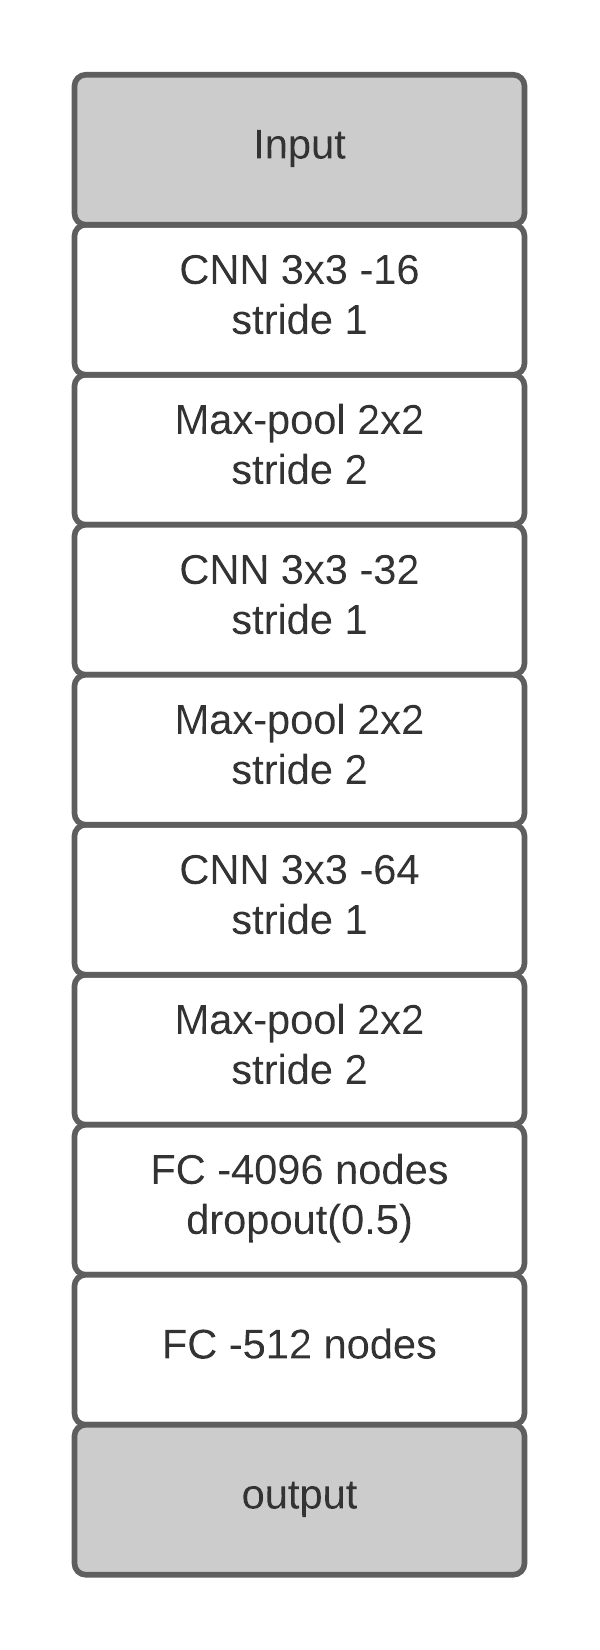
\includegraphics[scale=0.66]{../code/images/Net1_layers.png}  
	  \caption{Net1}
	\end{subfigure}
	\begin{subfigure}[t]{.23\textwidth}
	  \centering
	  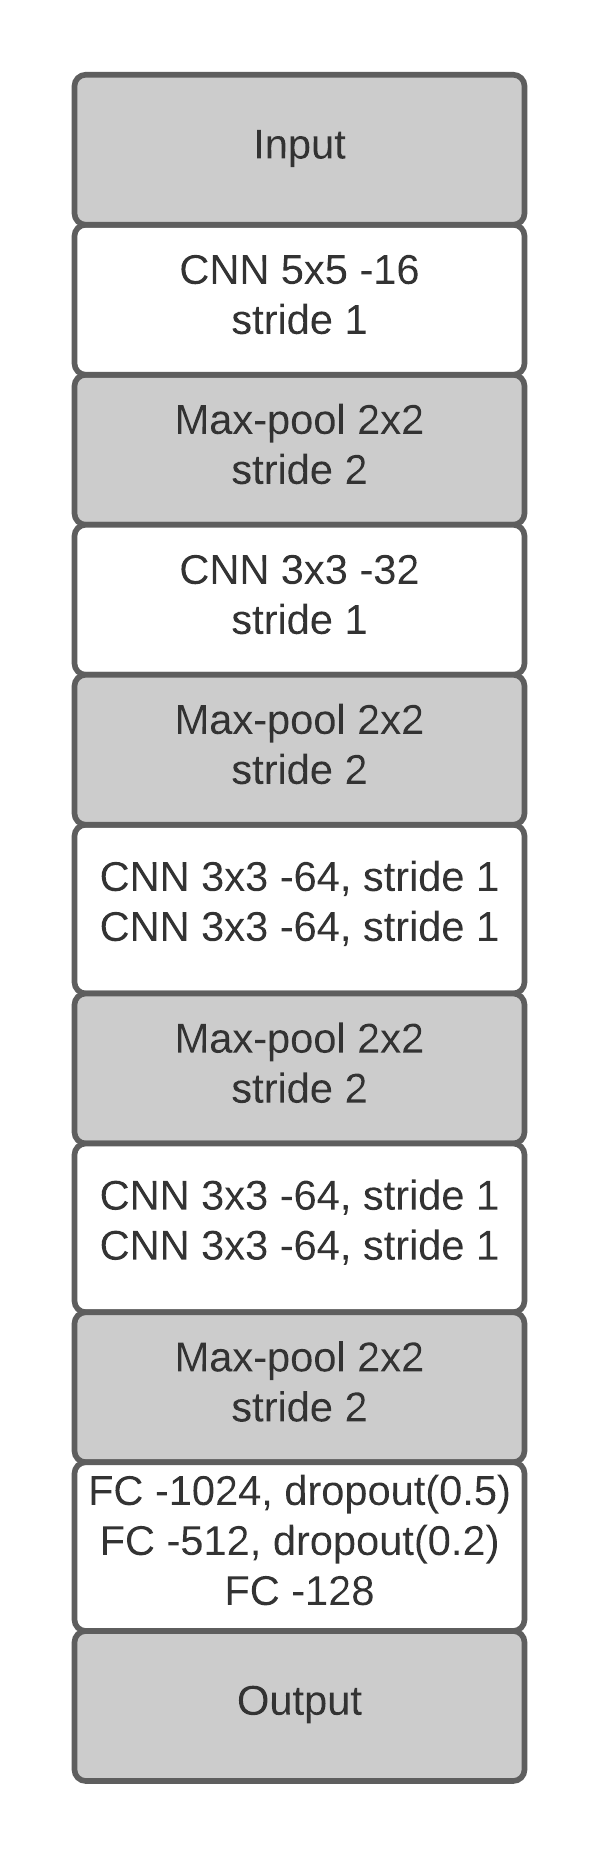
\includegraphics[scale=0.66]{../code/images/Net2_layers.png}  
	  \caption{Net2}
	\end{subfigure}
	\begin{subfigure}[t]{.23\textwidth}
	\centering
	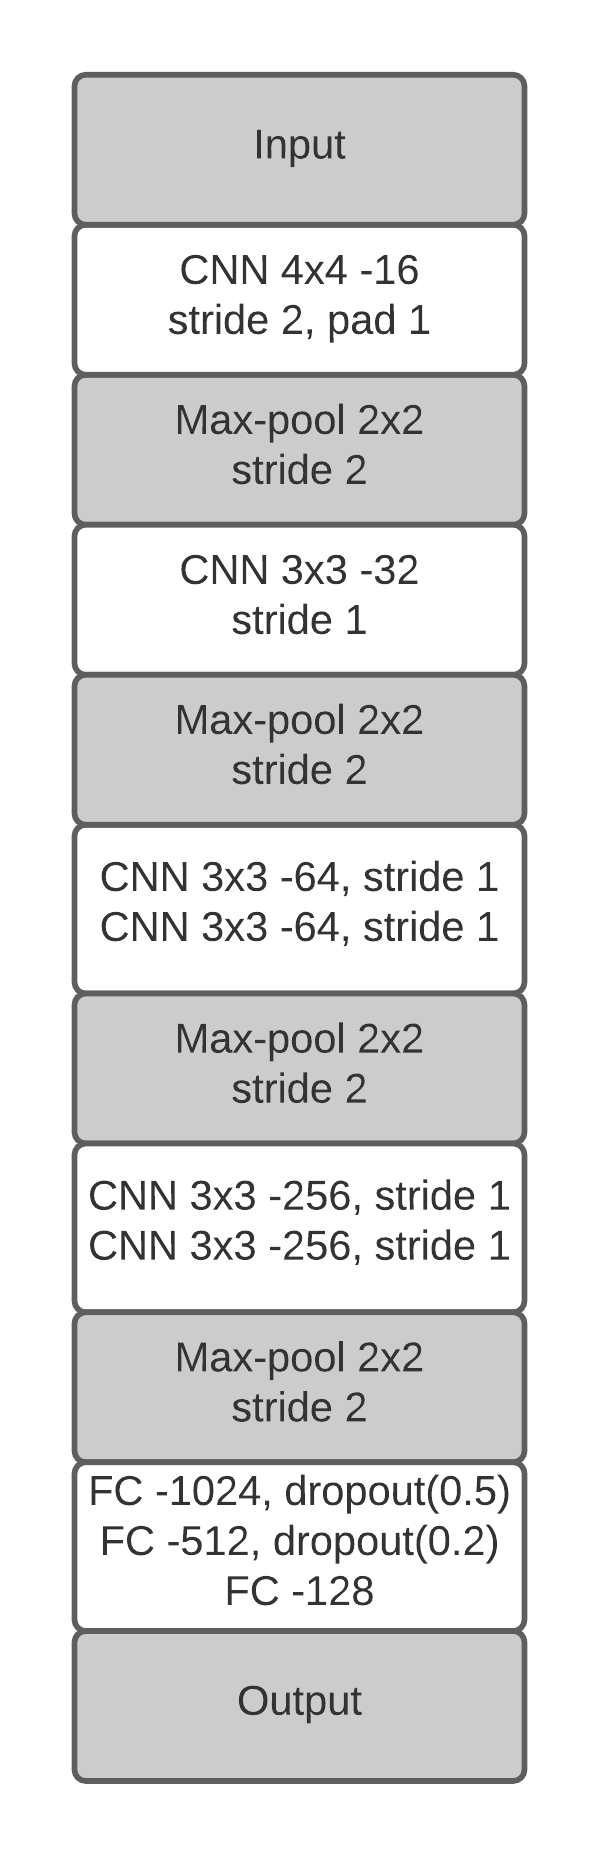
\includegraphics[scale=0.66]{../code/images/Net3_layers.png}
	\caption{Net3}		
	\end{subfigure}
	\begin{subfigure}[t]{.23\textwidth}
		\centering
		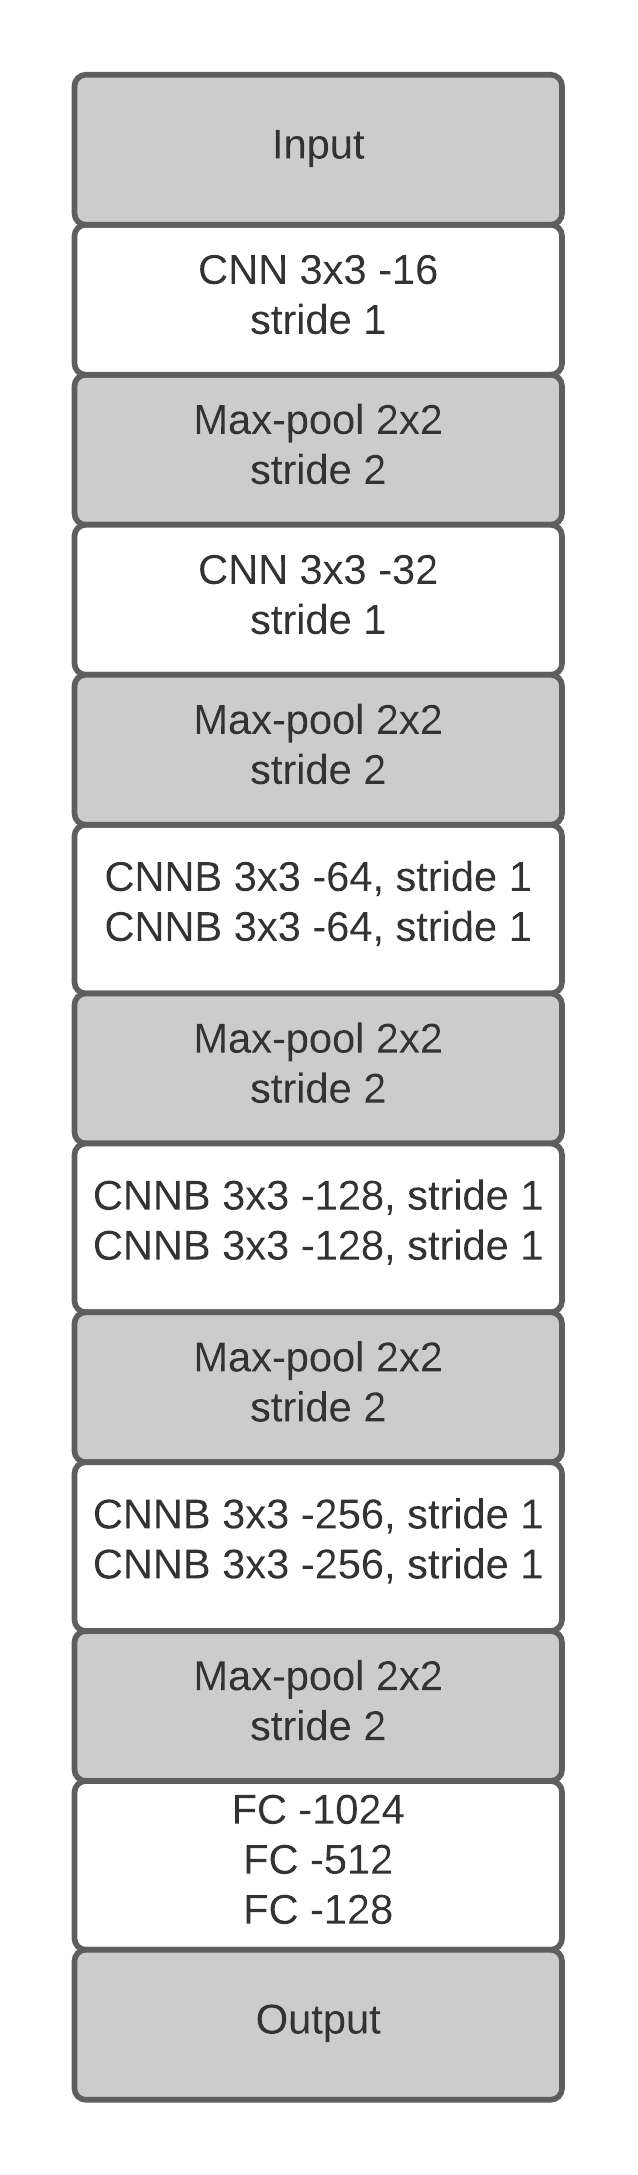
\includegraphics[scale=0.66]{../code/images/Net4_layers.png}
		\caption{Net4}		
		\end{subfigure}
	\caption{Summary of all trained models. CNNB refers to batch normalization before applying ReLU}
	\label{fig:models}
\end{figure}
\clearpage
\subsection{Training Results}
The following accuracy results were obtained after training all $4$ models, which were trained for a total of $50$ epochs. Each model was checkpointed every $10$ epochs, and the model with the best test accuracy was chosen as the final model for Part-B. The accuracies for all models are captured in \cref{table:test-acc}. The loss curve for the best performing model(Net 4) is present in \cref{fig:net4loss}.
\begin{table}[ht]
	\caption{Test and Validation Accuracy Chart(for all 4 models)}% title of Table
	\centering % used for centering table
	\begin{tabular}{|c | c | c | c|}% centered columns (4 columns)
		\hline\hline      
		Model & epochs & validation accuracy(\%) & test accuracy(\%) \\ [0.5ex]
		\hline  
		Net1&              10 &           70.16 &          70.28 \\
			&              20 &           75.88 &          74.64 \\
			&              30 &           78.16 &           76.2 \\
			&              40 &           76.92 &          76.68 \\
			&              50 &            77.8 &          77.16 \\
		\hline
		Net2&              10 &          36.04  &         35.84 \\
			&              20 &          63.12  &         61.44 \\
			&              30 &          73.56  &         70.32 \\
			&              40 &          76.16  &         73.16 \\
			&              50 &           79.4  &         76.16 \\
		\hline
		Net3&              10 &          39.84 &           39.6 \\
			&              20 &           61.2 &           59.4 \\
			&              30 &          70.24 &          69.16 \\
			&              40 &          75.84 &          74.44 \\
			&              50 &          77.32 &          75.48 \\
		\hline
		Net4&              10 &           78.2 &          76.96 \\
			&              20 &           81.4 &          79.92 \\
			&              \textbf{30} &           \textbf{83.4} &          \textbf{82.24} \\
			&              40 &          83.84 &           82.2 \\
			&              50 &          83.48 &          81.96 \\[1ex]
		\hline
	\end{tabular}
	\label{table:test-acc}% is used to refer this table in the text
\end{table}

\begin{figure}[ht]
	\centering
	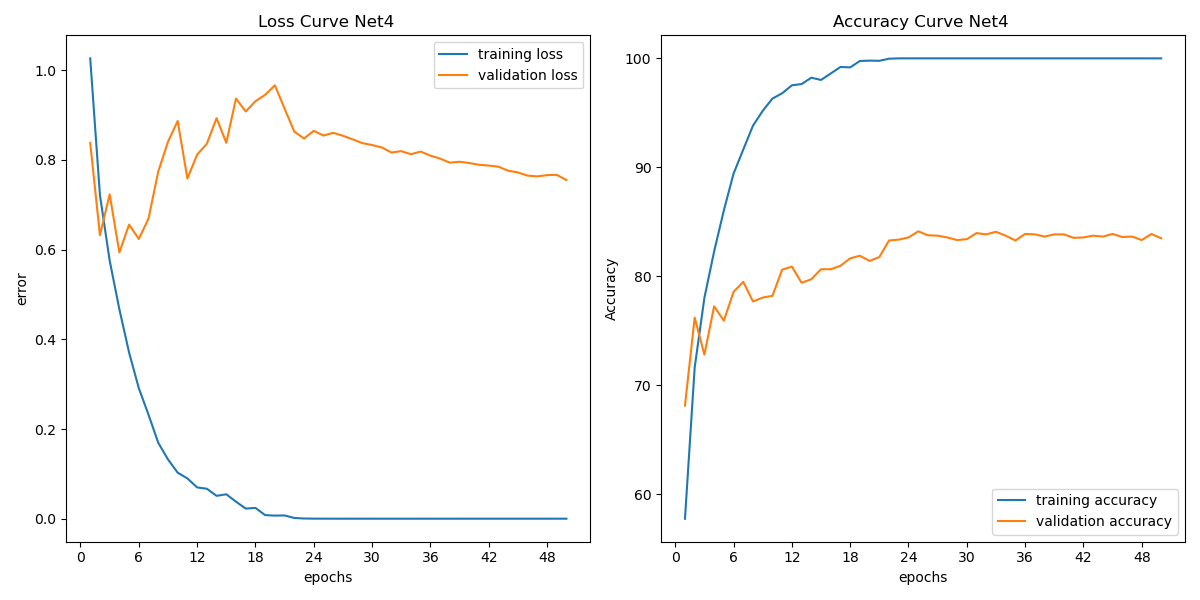
\includegraphics[scale=0.35]{../code/images/Net4.png}
	\caption{Loss curves for Net 4 (best model)}
	\label{fig:net4loss}
\end{figure}

\begin{table}[ht]
	\caption{Classwise accuracy on test dataset for Net4 - $30$ epochs}
	\centering
	\begin{tabular}{|c | c|}
		\hline\hline
		Class & Accuracy(in \%) \\ [0.5ex]
		\hline
		 aeroplane & 96 \\
		       cat & 65 \\
		      deer & 88 \\
		       dog & 70 \\
			  frog & 84 \\ [1ex]
		\hline
	\end{tabular}
\end{table}
\subsection{Training Inferences}
From the figures in \cref{table:test-acc} and the models in \cref{fig:models}, we can make the following conclusions about hyperparameter effects on performance:
\begin{enumerate}
	\item \textbf{Convolutional Layers}: In general, an increase in the number of convolutional layers lead to better train and test accuracy. However, for networks with very large number of conv layers, the train speed is very slow(as evidenced in Net2 and Net3). This can be offset by applying batch normalization after every conv layer(as evidenced in Net4).
	\item \textbf{No of filters/layer}: In general, having more number of filters in higher layers helped capture more detailed features, and led to a higher accuracy(as evidenced in Net3 and Net4)
	\item \textbf{Stride}: Convolving with stride $\geq 1$ seems to result in a reduced accuracy, as evidenced between Net2 and Net3. This happens because we miss out on features when increasing stride.
	\item \textbf{Maxpooling}: Increasing no of maxpooling layers in shallow nets(Net1) leads to greater loss.
\end{enumerate}
In \cref{fig:misclf5}, we can see a small subset of the misclassified images in the dataset split. In most of the images, it is hard to classify the images even with the naked eye.
\begin{figure}[ht]
	\centering
	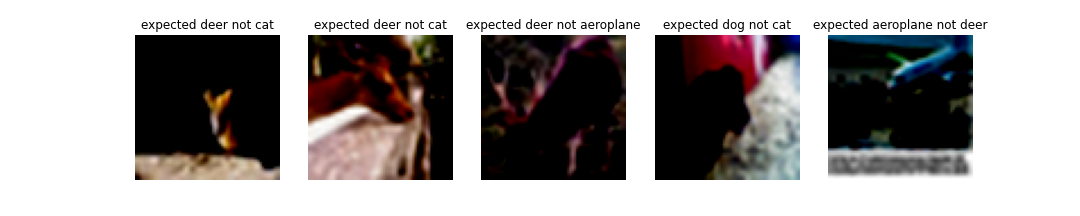
\includegraphics[scale=0.4]{../code/images/misclassified_imgs.png}
	\caption{Some misclassified images}
	\label{fig:misclf5}
\end{figure}

\section{Part-B}
For this part, all experiments are conducted with the weights learned after epoch $30$ of Net4 from Part-A. 
\subsection{Occlusion sensitivity experiment}
Occlusion experiments were carried out on $5$ random samples from the dataset, with a window size of $10 \times 10$ and $20 \times 20$ respectively. Some example images are visualized in \cref{fig:occhmps}.\\
From the heatmap outputs, we can infer that increasing the occlusion kernel size around the main features of the objects to be classified causes the probability of misclassification to increase(increase in blue shading).
\begin{figure}[t]
	\centering
	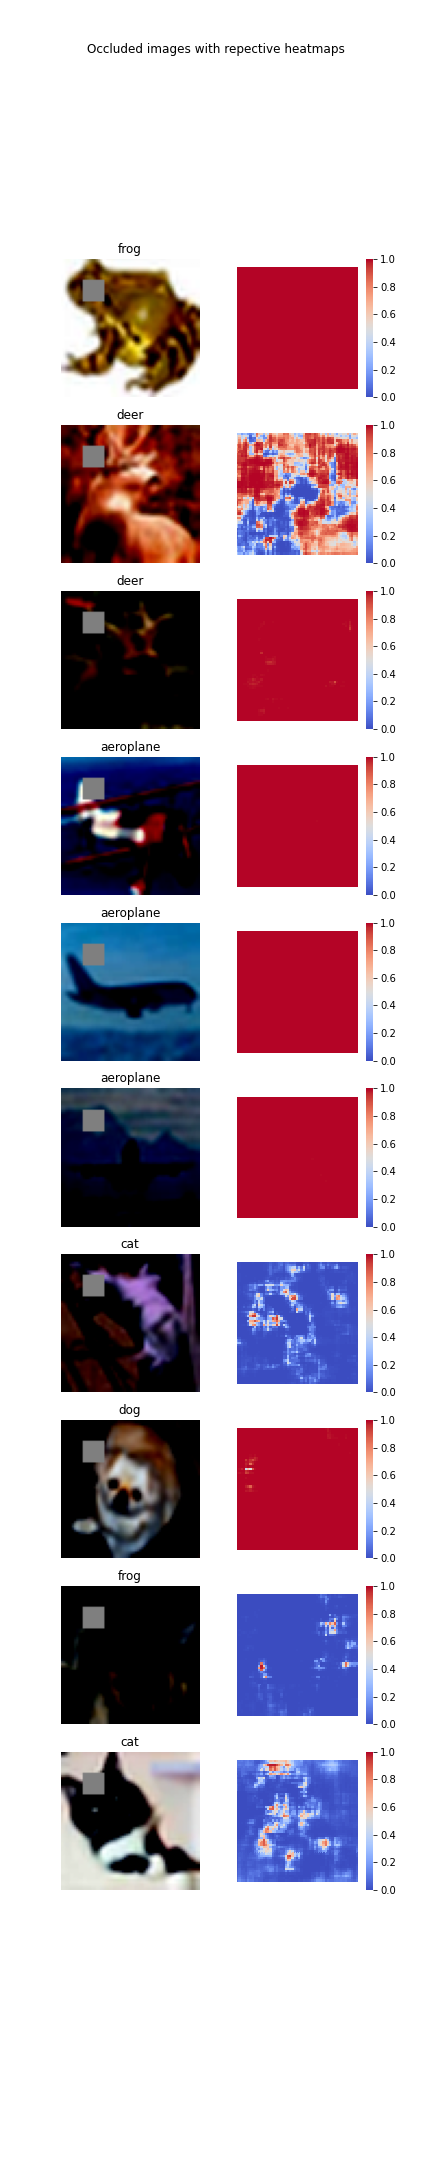
\includegraphics[scale=0.4]{../code/images/Occlusion_heatmaps.png}
	\caption{Images with probability heatmaps for kernels of size $10 \times 10$ and $20 \times 20$ for the occlusion sensitivity experiment}
	\label{fig:occhmps}
\end{figure}
\begin{table}[ht]
	\caption{Filter Selection in Net4}
	\centering
	\begin{tabular}{|c | c|}
		\hline\hline
		Conv Layer(sub-block \#) & Filter \#s \\ [0.5ex]
		\hline
		1 &   2 , 13 \\
		2 &  11 , 23 \\
		3-1 &   9 , 49 \\
		4-1 &  54 , 98 \\
		5-1 &   5 , 171\\ [1ex]
		\hline
	\end{tabular}
	\label{table:filtt}
\end{table}
\pagebreak

\subsection{Filter Analysis}
\subsubsection{Filter Identification}
In Net 4, the filters specified in \cref{table:filtt} were selected for further analysis. Some of these selected filters are visualized in \cref{fig:c1f13} to \cref{fig:c5f171}.

\begin{figure}[h!]
	\centering
	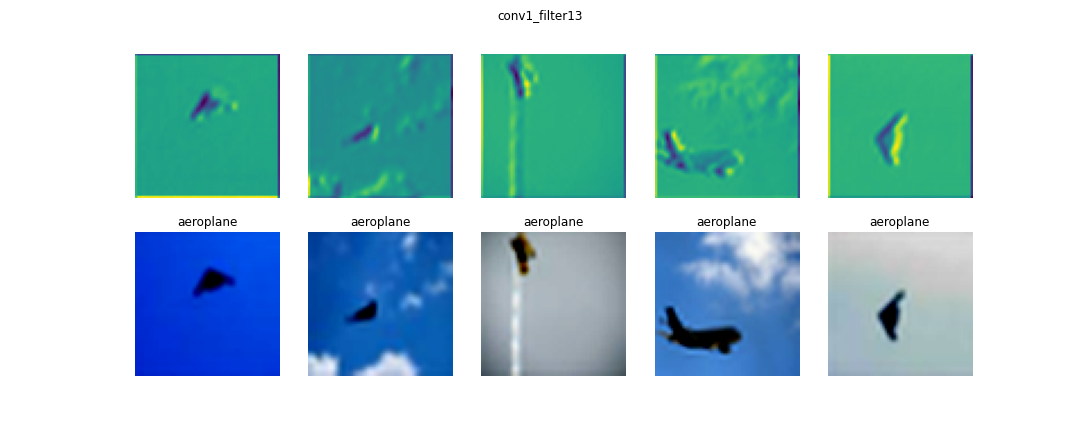
\includegraphics[scale=0.4]{../code/images/Filter_conv1_filter13.png}
	\caption{$13^{th}$ filter output corresponding to $1^{st}$ conv layer of Net4}
	\label{fig:c1f13}
\end{figure}

\begin{figure}[ht]
	\centering
	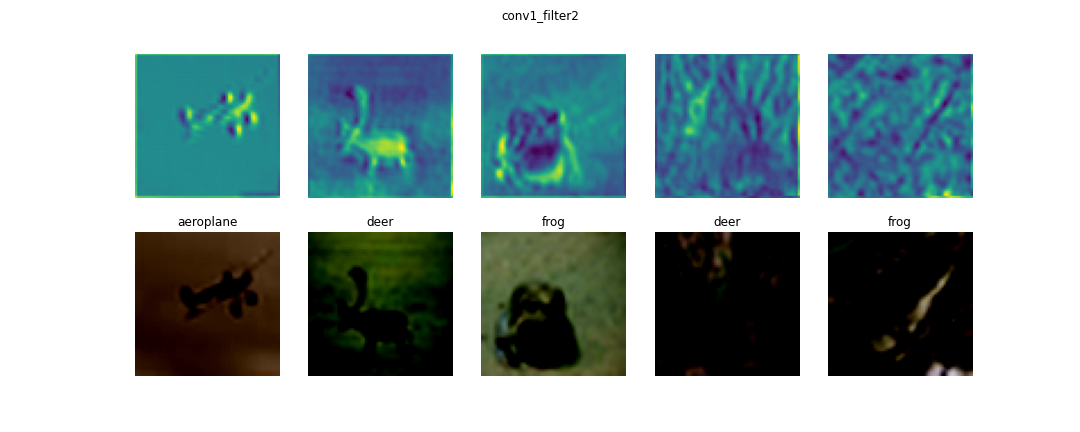
\includegraphics[scale=0.4]{../code/images/Filter_conv1_filter2.png}
	\caption{$2^{nd}$ filter output corresponding to $1^{st}$ conv layer of Net4}
	\label{fig:c1f2}
\end{figure}

\begin{figure}[ht]
	\centering
	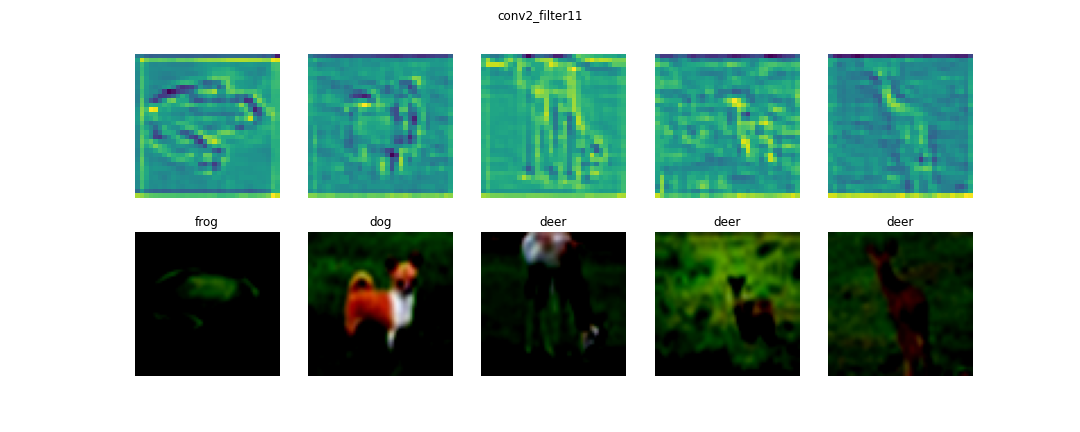
\includegraphics[scale=0.4]{../code/images/Filter_conv2_filter11.png}
	\caption{$12^{th}$ filter output corresponding to $2^{nd}$ conv layer of Net4}
	\label{fig:c2f11}
\end{figure}

\begin{figure}[ht]
	\centering
	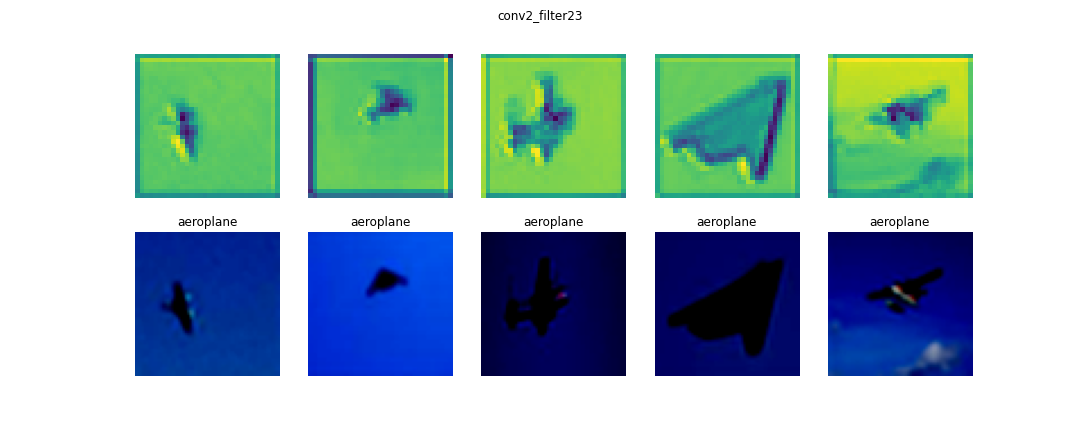
\includegraphics[scale=0.4]{../code/images/Filter_conv2_filter23.png}
	\caption{$23^{rd}$ filter output corresponding to $2^{nd}$ conv layer of Net4}
	\label{fig:c2f23}
\end{figure}

\begin{figure}[ht]
	\centering
	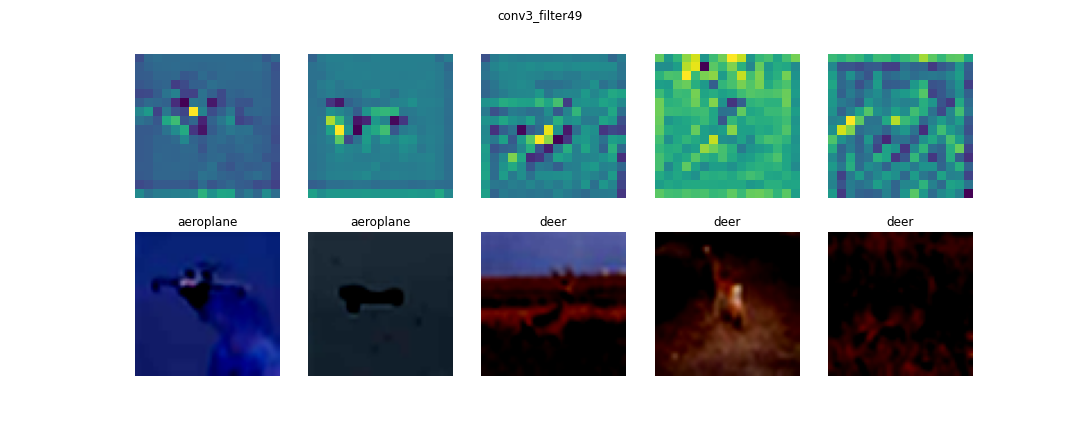
\includegraphics[scale=0.4]{../code/images/Filter_conv3_filter49.png}
	\caption{$49^{th}$ filter output corresponding to $3^{rd}$ conv layer of Net4}
	\label{fig:c3f49}
\end{figure}

\begin{figure}[ht]
	\centering
	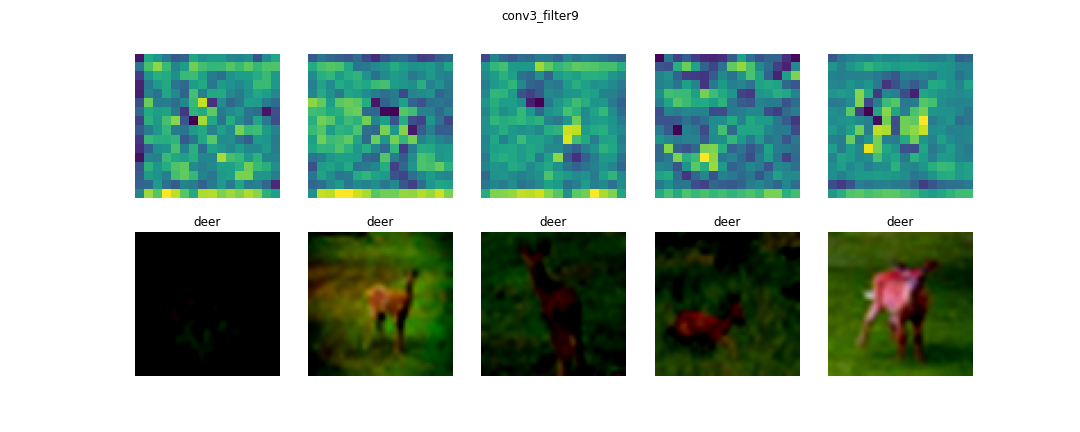
\includegraphics[scale=0.4]{../code/images/Filter_conv3_filter9.png}
	\caption{$9^{th}$ filter output corresponding to $3^{rd}$ conv layer of Net4}
	\label{fig:c3f9}
\end{figure}

\begin{figure}[ht]
	\centering
	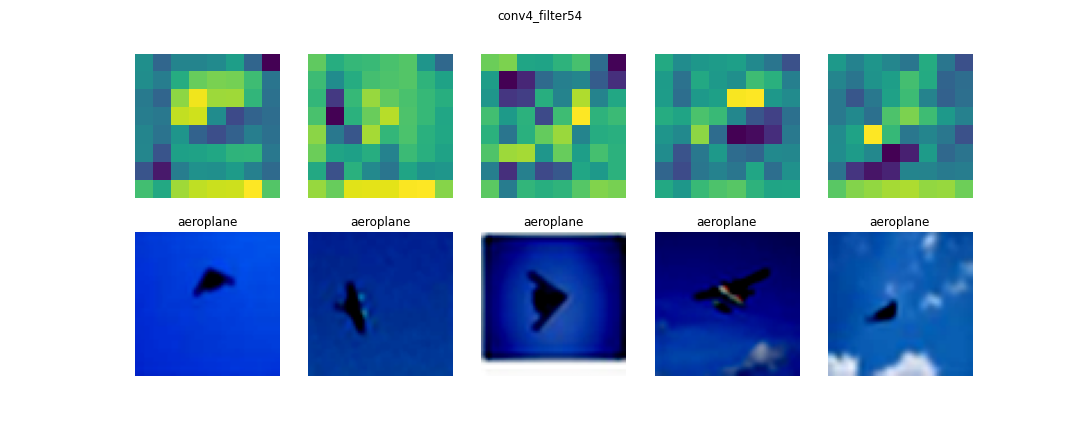
\includegraphics[scale=0.4]{../code/images/Filter_conv4_filter54.png}
	\caption{$4^{th}$ filter output corresponding to $54^{th}$ conv layer of Net4}
	\label{fig:c4f54}
\end{figure}

\begin{figure}[ht]
	\centering
	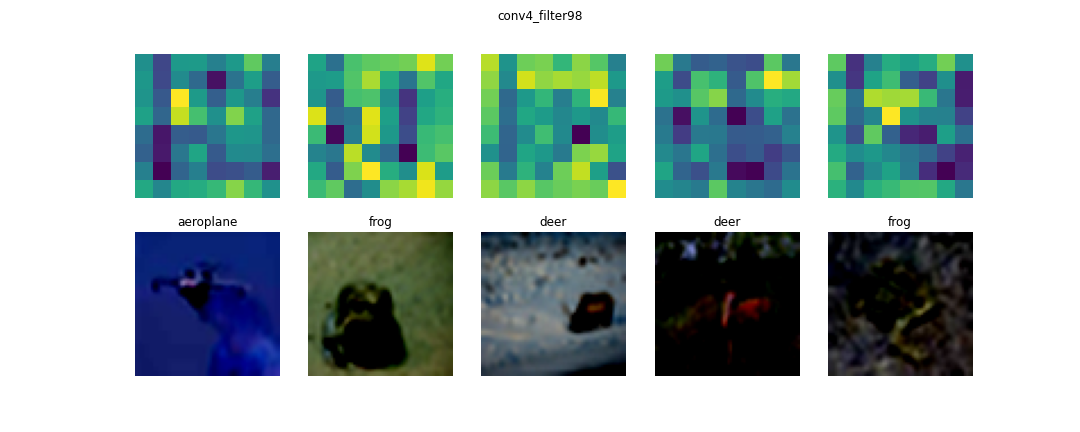
\includegraphics[scale=0.4]{../code/images/Filter_conv4_filter98.png}
	\caption{$4^{th}$ filter output corresponding to $98^{th}$ conv layer of Net4}
	\label{fig:c4f98}
\end{figure}

\begin{figure}[ht]
	\centering
	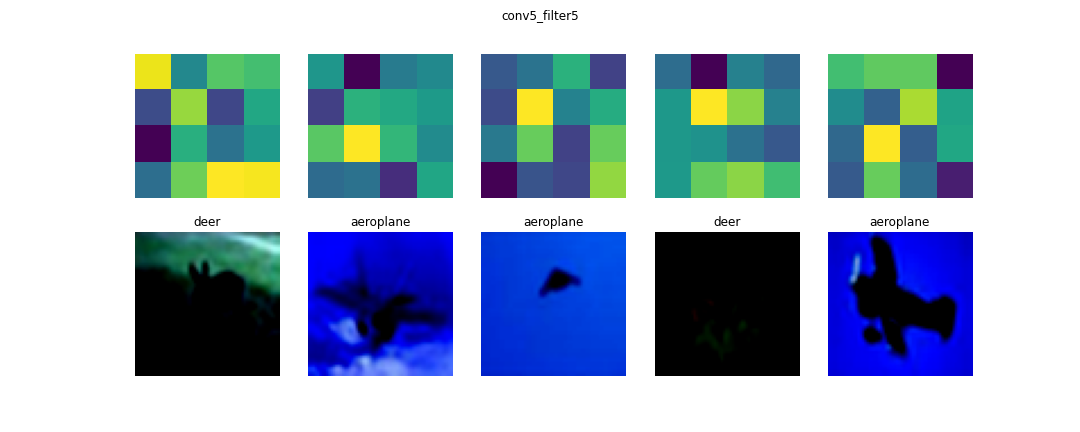
\includegraphics[scale=0.4]{../code/images/Filter_conv5_filter5.png}
	\caption{$5^{th}$ filter output corresponding to $5^{th}$ conv layer of Net4}
	\label{fig:c5f5}
\end{figure}

\begin{figure}[ht]
	\centering
	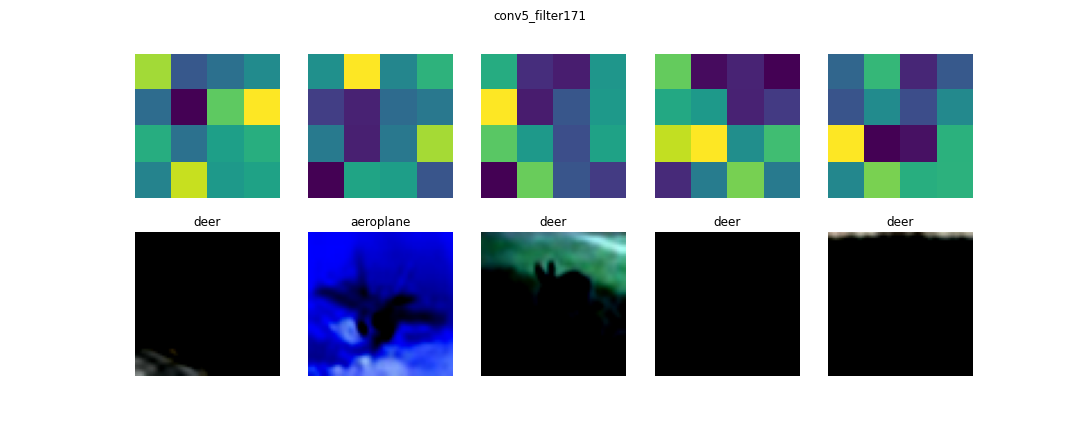
\includegraphics[scale=0.4]{../code/images/Filter_conv5_filter171.png}
	\caption{$171^{st}$ filter output corresponding to $5^{th}$ conv layer of Net4}
	\label{fig:c5f171}
\end{figure}
\clearpage
\subsubsection{Filter Modification}
The stats of the images which mis-classify after switching off the weights of the filters specified in \cref{table:filtt} is captured in \cref{table:miscimgs}\\
\begin{table}[h!]
	\caption{Misclassified image breakup after switching off filters present in \cref{table:filtt}}
	\centering
	\begin{tabular}{|c | c|}
		\hline\hline
		Class & Misclassification count \\ [0.5ex]
		\hline
		 aeroplane & 7 \\
		       cat & 31 \\
		      deer & 18 \\
		       dog & 50 \\
			  frog & 12 \\ [1ex]
		\hline
	\end{tabular}
	\label{table:miscimgs}
\end{table}
By viewing the values in \cref{table:miscimgs}, we can roughly conclude that the net effect of the filters in \cref{table:filtt} is to identify a common feature among cats, dogs and deers, which might be a form of quadrupedalism.\\
\cref{fig:reclfgimgs} shows some of the reclassified images after switching off the weights in \cref{table:filtt}.
\begin{figure}[ht]
	\centering
	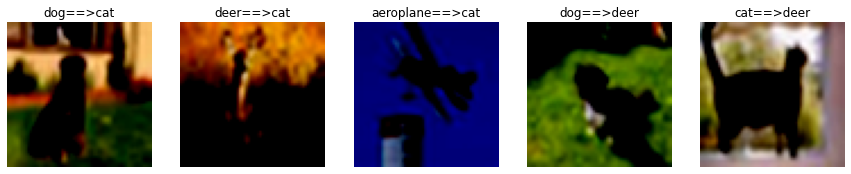
\includegraphics[scale=0.5]{../code/images/misclassified_switchoff.png}
	\caption{Some sample images reclasified after switching off weights}
	\label{fig:reclfgimgs}
\end{figure}
\end{document}
